\documentclass{article}

\renewcommand\refname{Referencias}
\renewcommand{\figurename}{Figura}

\usepackage{graphicx}
\graphicspath{{images/}}
\usepackage{floatrow}

\title{CouchDB: Investigación e implemetanción demostrativa de una base de datos NoSQL}
\author{Sebastián Hurtado \and Diego Linares \and Piero Marini}
\date{28 de Noviembre del 2019}

\begin{document}
    \maketitle  
    \section{Introducción}
        El objetivo de la presente investigación es entender el funcionamiento de una base de datos NoSQL y realizar una demostración de esta con una colección de datos. Actualmente, la data que resulta del uso en particular de aplicaciones web, redes sociales, etc. se encuentra en un nivel bajo de estructuración. Como resultado de ello, el uso de base de datos relacionales puede no ser el más adecuado para trabajar con este tipo de data \cite{sangeeta}. En este caso, exploraremos una de las soluciones NoSQL, que provee soporte ACID y permite trabajar con data no estructurada en formato JSON, CouchDB. \\
        El siguiente artículo se va a encontrar dividido de la siguiente manera: primero se definirá CouchDB y se comparará frente a otras soluciones de este tipo, observando en que casos conviene el uso del primero. A continuación explicaremos más a detalle las características del modelo de datos y la arquitectura de almacenamiento distribuido. Finalmente se hará una demostración de su uso en una colección de datos del servicio web Yelp, y se realizarán conclusiones en base a la misma. 
        \subsection{Definición y Propósito}
            CouchDB es un \textit{cross-platform, open-source}, base de datos de tipo NoSQL. Su arquitectura interna se encuentra diseñada específicamente para la web, y permite trabajar con grandes cantidades de data. Este hace uso de un \textbf{Couch Replication Protocol} para sincronizar documentos JSON entre 2 pares a través de un protocolo HTTP. Por ejemplo, los \textit{requests} son realizados a una determinada URL para obtener información con respecto a las bases de datos que se están manejando. Esto permite hacer uso de \textit{CURL} o cualquier otro intérprete para trabajar con los archivos que se encuentran en una base de datos CouchDB. \\
            Las bases de datos de CouchDB almacenan los llamados \textbf{documentos}. Estos consisten de un número variable de campos, los cuales pueden ser de diversos tipos, en conjunto con su metadata. Las ediciones por parte del cliente son realizadas a través de una carga, modificación y guardarlos de vuelta. Las transacciones son de estilo \textit{todo o nada}, por lo cual en la base de datos nunca se van a encontrar documeentos parcialmente editados. \\
            Un aspecto que diferencia a CouchDB de otras base de datos NoSQL es el mantenimiento de las propiedades ACID de una transacción. Las actualizaciones de documentos son serializadas, mientras que las lecturas de los mismos se realizan de forma concurrente. Para esta concurrencia es usado un \textit{Multi-Version Concurrency Control}, en el cual cada usuario ve una etapa constante de la base de datos de inicio a fin. La estructura de datos utilizada para organizar los datos es un B-Tree. Las actualización ocurren hasta el final de una transacción, dejando la base de datos en un estado consistente. \\
            El propósito de CouchDB, es el de trabajar con data no estructurada, particularmente para la web. Hacen uso del paradigma \textit{map-reduce}, replicación fácil y una \textit{straightforward RESTful API} \cite{lerner}. Como resultado de ello resulta útil para un ambiente de producción web. Además de las previas razones para ello, se le suma el echo de que toma de la arquitectura de la web (en palabras del desarrollador de Django \textit{``It's built of the web''}). Otras ventajas particulares son su alta escalabilidad y la ya mencionada facilidad de replicación. 
        \subsection{Cuadro comparativo con otras BD NoSQL}
            Las prinicipales diferencias de CouchDB son 3: el lenguaje de implementación en el que se encuentra (Erlang), el modelo de datos que usa (JSON), y la carencia de un lenguaje de queries fijo.\\
            \begin{figure}[h]
                \caption{Cuadro comparativo de diferentes tipos de bases de datos NoSQL, tomada de \cite{sandeep}.}
                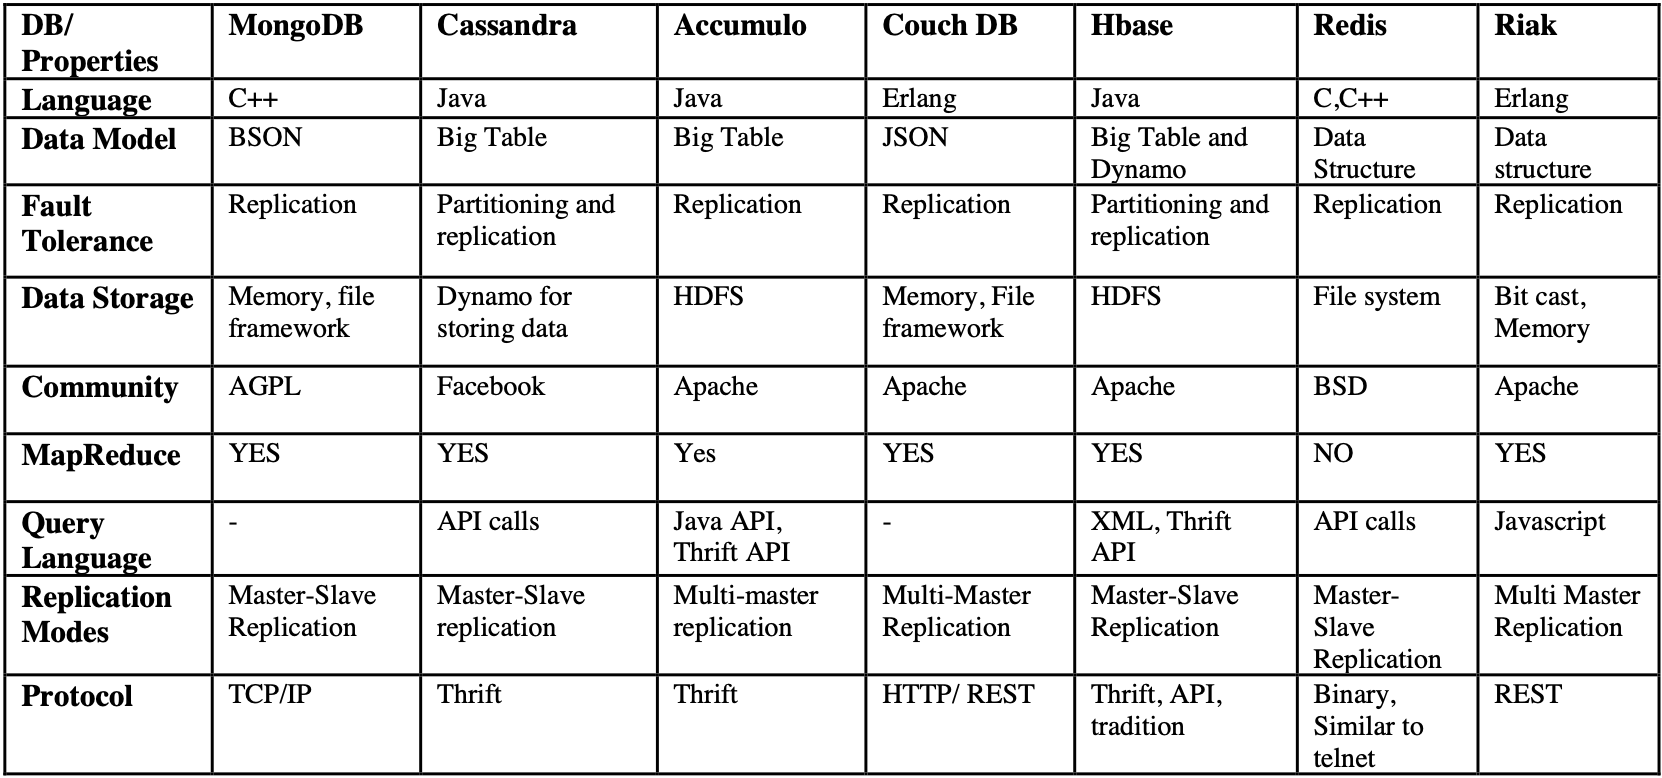
\includegraphics[width = \textwidth]{comparisonTable.png}
            \end{figure}
            El beneficio del uso de Erlang es que este se encuentra priorizado para \textit{fault tolerance} y en segunda medida, para concurrencia. Como se mencionó anteriormente, los documentos de CouchDB se encuentran guardados en formato JSON, que se encuentra directamente relacionado con su sistema de views. El protocolo del mismo se encuentra basado en JSON, en conjunto con servidores de socket externo; además de no haber límite para el \textit{text-size} o número de elementos de cada documento. CouchDB carece de soporte para un lenguaje de queries declarativo, en cambio, estas son basadas en REST/HTTP. Los requests son hechos de forma directa a una URL, lo cual permite realizar pruebas de queries de forma directa, y que el acceso a las bases de datos sea estandarizado. 
        \subsection{Escenarios de uso}
            Es necesario considerar que CouchDB, actualmente, tiene un relativo pequeño campo de mercado (usado por 3900 empresas) en comparación a otras bases de datos NoSQL. Es utilizado en casos de manejo de grandes volúmenes de data y almacenamiento basado en la nube. Razón para ello es su alta escabilidad (las BDR tienden a no soportar más de 1024 columnas de forma estable). Muchas de sus aplicaciones toman ventaja de la replicación y \textit{attachment management features} que son específicas de CouchDB \cite{rascovsky}. Los ámbitos en los cuales esto es aplicable son varios ámbitos, el mismo \cite{rascovsky} lo menciona en el caso de hospitales de radiología.\\
            Además, CouchDB ofrece beneficios particulares para portales y gateways \cite{hanlon}, gracias a que provee un API RESTful. Permite un acceso a data más rápido para los usuarios. Uno de los costos de esto, y debe ser tomado en consideración para el uso de CouchDB, es espacio adicional en disco disponiblee. Esto es debido a que sus índices Btree y los views se encuentran almacenados en este. Uno de los ejemplos, de este beneficio estuvo presente en el portal de usuarios de Teragrid en el cual se logró un aumento de velocidad de 8.24x \cite{hanlon} para permitir que la información se encuentre mucho más disponible al usuario.
    \section{Características}
        \subsection{Modelo de datos}
            \subsubsection{Inserciones}
            \subsubsection{Actualizaciones}
            \subsubsection{Búsqueda}
            \subsubsection{Indexación} 
        \subsection{Arquitectura de almacenamiento distribuido}
            Es posible dividir la arquitectura de CouchDB en 3 componentes principales: engine de almacenamiento, engine de vistas, y replicador \cite{padhy}. El almacenamiento es basado en una estructura de \textit{BTree}, y accedidas por llave o rango (haciendo uso de las operaciones del árbol), de forma rápida. El engine de vistas se encuentra escrito en JavaScript, basado en jobs de MapReduce, por lo que sirve para indices y extracción de data. El replicador se conecta a bases de datos locales o remotas y las sincronizan. \\
            Las relaciones entre los componentes mencionados pueden ser observados en el siguiente gráfico. \\
            \begin{figure}[h]
                \caption{Gráfico de relación entre los componentes distribuidos de CouchDB, tomado de \cite{padhy}.}
                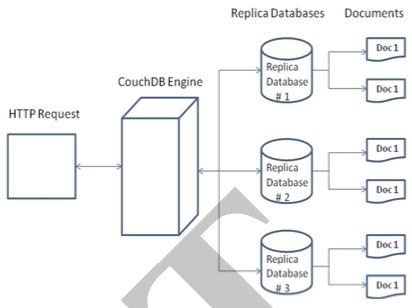
\includegraphics[width = 0.6\textwidth]{architecture.png}
            \end{figure}
            \subsubsection{Fragmentación, Asignación, Replicación}
                Las inserciones en CouchDB son realizadas en forma de \textit{append-only}, de forma que se evita la Fragmentación. Los appends son realizados al final del documento que se busca modificar. No hay una necesidad de realocación de memoria. De la misma manera, permite realizar compactación, a través de la escritura de un \textit{revision} a los archivos de una nueva base de datos (en la que incluye los documentos eliminados). Finalmente, la antigua base de datos es remplazada con la nueva que se encuentra compactada. \\ 
                La replicación se puede realizar de dos maneras, transiente, y persistente. Una replicación transiente se refiere a la carencia de un documento que sirva de backup durante la replicación; este hace uso del api endpoint \texttt{\_replicate}, y no permite realizar queries de su estado hasta que el trabajo se encuentre terminado. Las replicaciones persistentes mantienen un documento con los parametros de replicación utilzados, los cuales se guardan en una base de datos \texttt{\_replicator}, en donde cada documento describe un proceso tomando lugar. Las replicaciones funcionan comparando el objetivo con el source. Unicamente se transfieren aquellos documentos que difieren y se eliminan los que no se encuentran en la fuente. \\
                Una replicación finaliza cuando el stream de cambios se ha acabado, con algunos check-points realizado en medio en caso de fallas o caída del servidor. Las replicaciones son hechas en una única dirección por, lo cual es necesario dos procesos para realizar una replicación de master a master. \\
                De acuerdo a la documentación oficial de CouchDB, el control de documentos a replicar puede ser hecho a través de tres métodos: 
                \begin{enumerate}
                    \item Local: si los documentos son locales estos nunca se replican. 
                    \item Selector: se encuentran en los documentos de parámetro y contienen una query que determina si un determinado documento debe ser replicado o no. 
                    \item Funciones de filtrado: por cada uno de los documentos que se van a replicar, estos pasan por una función de filtrado, que en caso de retornar verdadero, continúan con el proceso. 
                \end{enumerate}
            \subsubsection{Procesamiento de consultas distribuidas}
                La computación distribuida es posible en CouchDB gracias al uso del modelo de programación MapReduce. Es esencialmente un patrón que permite implementar queries de gran escala para un motor de búsqueda \cite{sciabrra}. El mapeo produce valores que son clasificados a través de llaves, y el reduce agrega estos resultados. La función se encuentra embedida como parte de JavaScript. Esto significa que la base de datos hace la mayor parte del trabajo, mientras que el developer se debe enfocar en la extracción de la información. \\ 
                La arquitectura de quieres posee un feature conocido como \textit{direct shard connection only}, donde un \textit{shard} es una partición horizontal de data en la base de datos, con el objetivo de generar durabilidad. El componente que realiza la resolución del shard-key es el coordinador de queries. Una desventaja ed CouchDB, es que este no ofrece soporte para queries que usen non-shard key values. Por otra parte, el merge de los resultados múltiples provenientes de múltiples shards es también realizado por el coordinador de queries y enviado a cada uno de los clientes. El ordenamiento de estos resultados se encuentra soportado. \\ 
                Cabe resaltar la existencia de CouchDB Lounge, un paquete que permite clustering de nodos que reciben hashing constante. Este permite que estos nodos se mezclen de una forma más sencilla. Actualmente este se encuentra en proceso de traducción a Erlang para su integración en CouchDB regular. 
    \section{Implementación Demostrativa}
        \subsection{Carga de una colección de datos}
        \subsection{Consulta de datos de forma distribuida}
    \section{Conclusiones}

    \newpage

    \bibliographystyle{unsrt}
    \bibliography{bibliography}
\end{document}